\chapter{Evaluation}
To ensure that the prototype satisfied our final problem statement, some evaluation had to be done on the prototypes performance. As described in \autoref{sec:userTesting}, user testing had to be conducted, to evaluate whether the prototype performed as intended and to gather knowledge about what needed to be revised in future iterations.

\section{The usability test}
In order to find out to which degree our prototype met our usability requirements, we conducted a usability test.

\subsection{Test goals}
The main goal of this test was to figure out if our prototype had satisfactory usability, and if indeed did satisfy our usability requirements. These goals specifically included:\\
\begin{enumerate}
	\item Enough different plants to make a satisfactory garden for the client.\\
	\item The virtual environment should be pleasurable to be in.\\
	\item The garden architect should have control over the virtual objects with physical tokens.\\
\end{enumerate}


\subsection{Sampling}
With the initial test idea, the plan was to test on our main target group, with time constraints and transport resources not being possible, we ended up finding 8 participants, utilizing convenience sampling on AAU CPH.

\subsection{Test specifics}
In \autoref{fig:test1} seen below, is the setup for our usability test.

\begin{figure}[H]
	\centering
	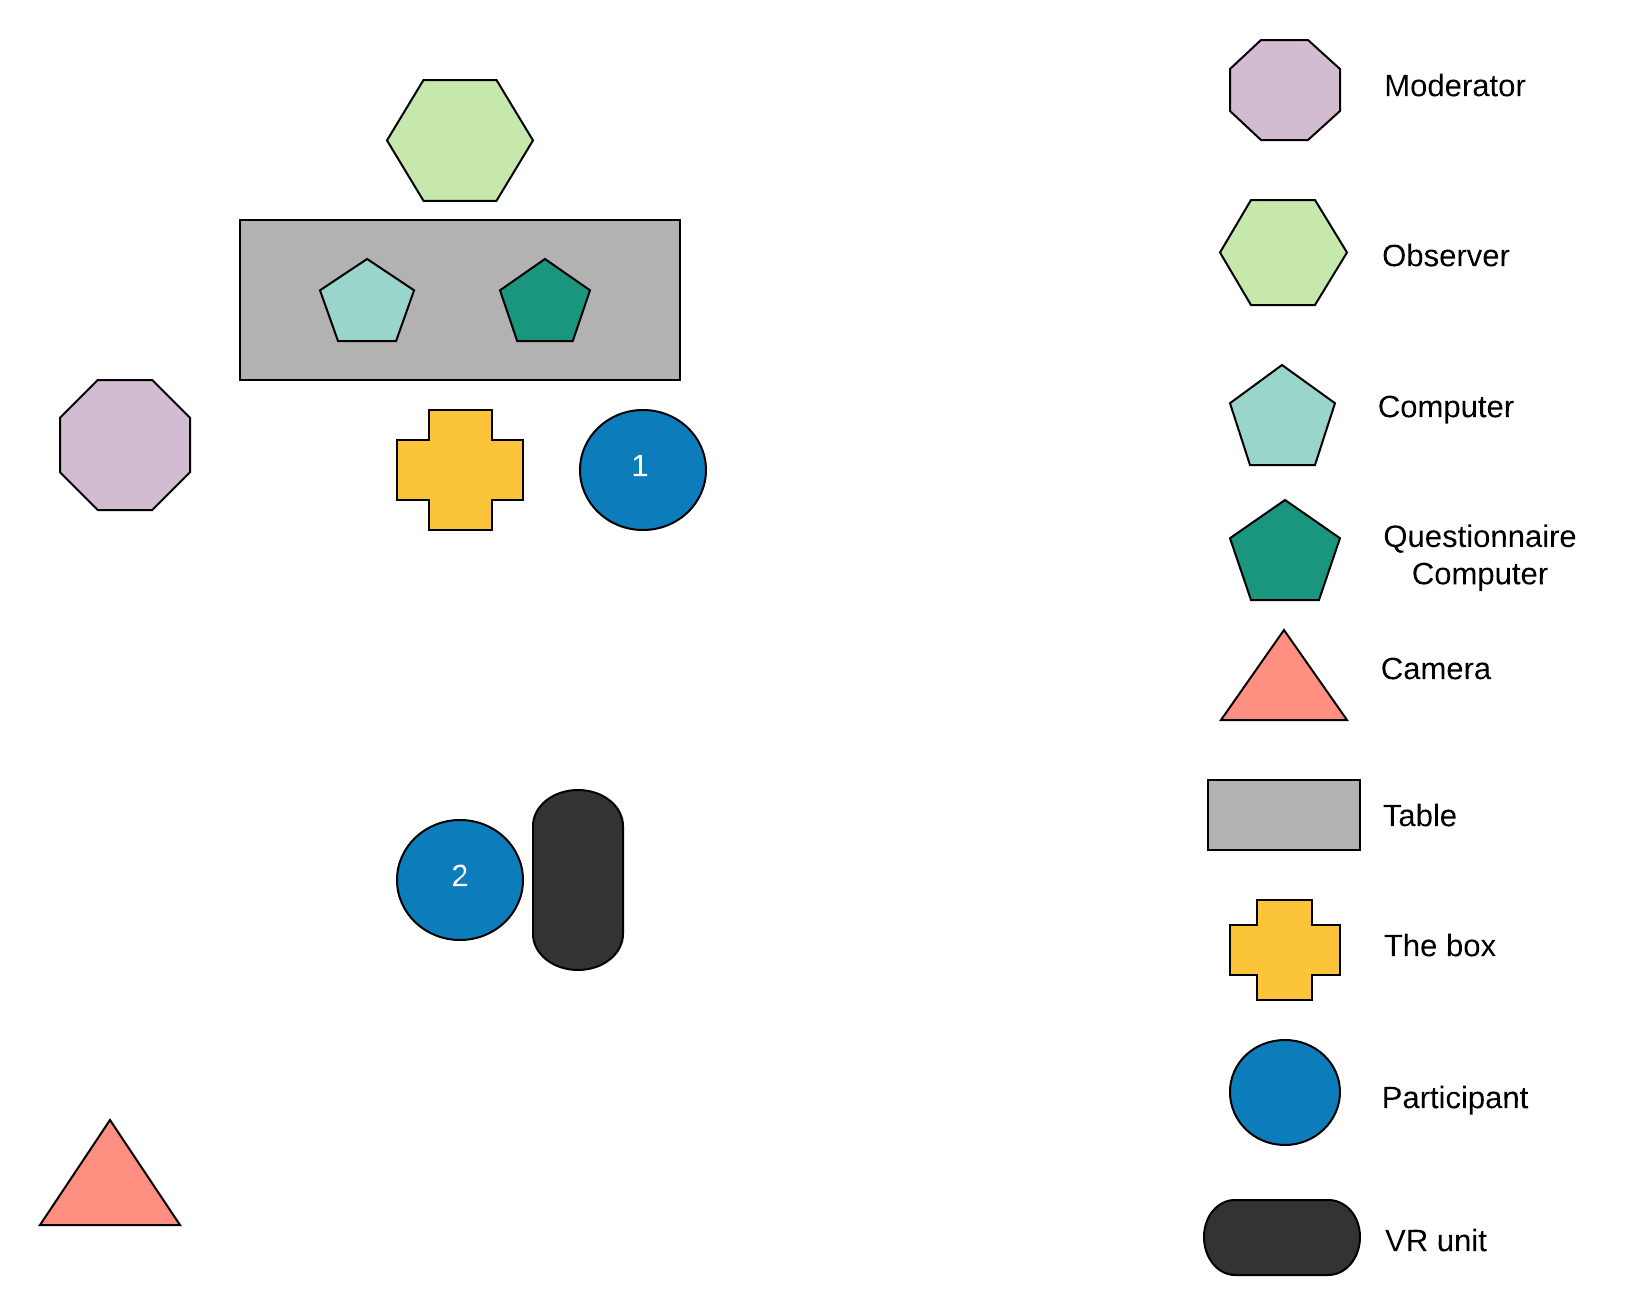
\includegraphics[width=1\linewidth]{figure/Evaluation/Test1.png}
	\caption{Our test setup, with the location of the participant, moderator, video camera and equipment. The two phases are visualized by the numbers in the circles.}
	\label{fig:test1}
\end{figure}

\subsection*{The equipment being used during the test}
\begin{itemize}
	\item[-] A camera running on a computer
	\item[-] The box where the tokens is placed with a camera inside
	\item[-] Laptop for filling out a questionnaire
	\item[-] HTC vive VR unit
\end{itemize}

\subsection*{Location and schedule}
The test took place Thursday 7/12 2017 in our group room at Aalborg University Copenhagen on Frederikskaj 12. Each testing with evaluation took approximately 15 to 20 minutes.

\subsection*{Test procedure}
Before the test began, the participant was informed about the general purpose of the test, tasks and their given consent to being recorded. After agreeing to this, the participant was asked to take the role of a client or an architect. Then they where asked to act like they were planning on having and designing a new garden and find out how the design should look like. The client would take on the VR goggles and the architect would make a design with the markers, with the help from the client. Afterwards the participants would switch roles and do the same thing again.

After the participants tried their different roles they where asked to fill out a questionnaire (\ref{sec:appendixUsability}) as their respective roles, so each participant had to fill out two questionnaires. The questionnaires contained questions regarding the experience as a client and an architect.

\subsection{Results}
In this section we will display the results conducted from our questionnaires that the participants filled out after each role in the test (see \autoref{fig:boxPlotResults} and \autoref{fig:boxPlotResults2}). Some of the questions will be picked out and shown in a bar chart.\\
The questions is as follows:\\

Client Questions:\\
\begin{enumerate}
\item Rate the amount of discomfort you experienced during the test.
\item Was the framerate (the frequency at which the screen updates) tolerable?
\item How engaged did you feel with the program?
\item How good did the environment and objects look?
\item Did you feel you had enough space to move around?
\item Could you easily communicate with the other participant?
\end{enumerate}


\begin{figure}[H]
	\centering
\begin{tikzpicture}
\begin{axis}
[
boxplot/draw direction=y,
height=7cm,
width=10cm,
enlargelimits=0.03,
ytick={1,1.5,2,2.5,3,3.5,4,4.5,5},
xtick={1,2,3,4,5,6},
xlabel=Questions,
ylabel={Level of agreement},
xticklabels={
	1,2,3,4,5,6}
]
\addplot+[boxplot]
table[row sep=\\,y index=0] {
	data\\ 1\\ 1\\ 1\\ 2\\ 2\\ 2\\ 3\\ 4\\
};
\addplot+[boxplot]
table[row sep=\\,y index=0] {
	data\\ 2\\ 2\\ 2\\ 3\\ 4\\ 5\\ 5\\ 5\\
};   
\addplot+[boxplot]
table[row sep=\\,y index=0] {
	data\\ 4\\ 4\\ 4\\ 4\\ 4\\ 4\\ 4\\ 5\\ 
};   
\addplot+[boxplot]
table[row sep=\\,y index=0] {
	data\\ 2\\ 3\\ 4\\ 4\\ 4\\ 5\\ 5\\ 5\\
};  
\addplot+[boxplot]
table[row sep=\\,y index=0] {
	data\\ 2\\ 2\\ 3\\ 3\\ 3\\ 5\\ 5\\ 5\\
};  
\addplot+[boxplot]
table[row sep=\\,y index=0] {
	data\\ 1\\ 1\\ 4\\ 5\\ 5\\ 5\\ 5\\ 5\\
};  
 
\end{axis}
\end{tikzpicture}
\caption{Box plot graph showing the result of the client scale questions.}
\label{fig:boxPlotResults}
\end{figure}

Architect questions:\\
\begin{enumerate}
	\item How easy was the product to use?
	\item How easy was it to tell what the garden looked while you were building it?\\
\end{enumerate}
\begin{figure}[H]
	\centering
	\begin{tikzpicture}
	\begin{axis}
	[
	boxplot/draw direction=y,
	height=7cm,
	width=10cm,
	enlargelimits=0.03,
	ytick={1,1.5,2,2.5,3,3.5,4,4.5,5},
	xtick={1,2},
	xlabel=Questions,
	ylabel={Level of agreement},
	xticklabels={
		1,2}
	]
	\addplot+[boxplot]
	table[row sep=\\,y index=0] {
		data\\ 1\\ 3\\ 3\\ 4\\ 4\\ 5\\ 5\\ 5\\
	};
	\addplot+[boxplot]
	table[row sep=\\,y index=0] {
		data\\ 1\\ 1\\ 2\\ 2\\ 2\\ 3\\ 3\\ 3\\
	};   
	
	
	\end{axis}
	\end{tikzpicture}
	\caption{Box plot graph showing the results of the architect scale questions.}
	\label{fig:boxPlotResults2}
\end{figure}

\subsection*{Was the framerate (the frequency at which the screen updates) tolerable?}
As seen in \autoref{fig:barChartFrame}, 3 of the 8 participants didn't find the framerate very tolerable. 1 participant found it somewhat tolerable and 3 participants found it very tolerable.

\begin{figure}[H]
	\centering
	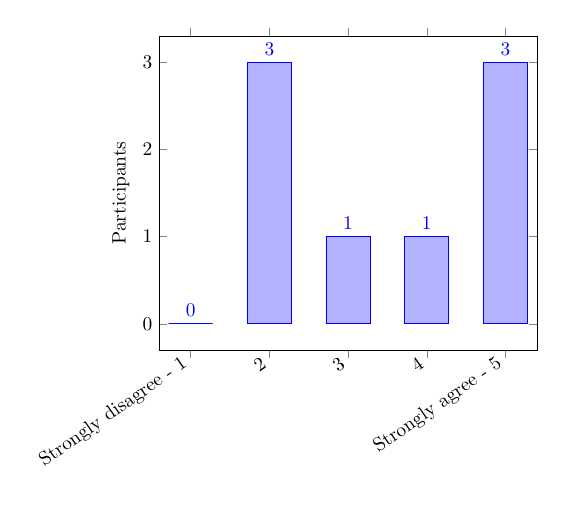
\begin{tikzpicture}[scale=0.7]
	\begin{axis}[ybar,bar width=0.8cm,enlargelimits=0.1,legend style={at={(0.5,-0.2)},anchor=north,legend columns=-1},ylabel={Participants},symbolic x coords={Strongly disagree - 1,2,3,4,Strongly agree - 5},xtick=data,nodes near coords,nodes near coords align={vertical},x tick label style={rotate=35,anchor=east},]
	\addplot coordinates {(Strongly disagree - 1,0) (2,3) (3,1) (4,1) (Strongly agree - 5,3)};
	\end{axis}
	
	\end{tikzpicture}
	\caption{Bar chart showing if the participants found the framerate tolerable.}
	\label{fig:barChartFrame}
\end{figure}

\subsection*{How easy was the product to use?}
Out of 8 participants 1 of them strongly disagreed that the product was easy to use, while 2 participants hit the middle ground and 5 participants agreed that the product was easy to use. This can be seen in \autoref{fig:barChartEasy}.

\begin{figure}[H]
	\centering
	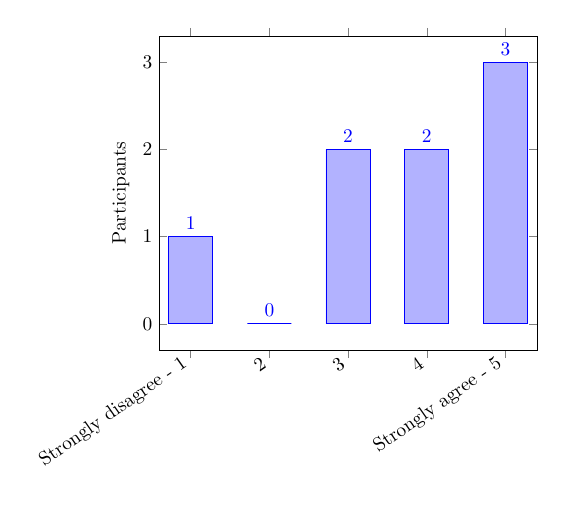
\begin{tikzpicture}[scale=0.7]
	\begin{axis}[ybar,bar width=0.8cm,enlargelimits=0.1,legend style={at={(0.5,-0.2)},anchor=north,legend columns=-1},ylabel={Participants},symbolic x coords={Strongly disagree - 1,2,3,4,Strongly agree - 5},xtick=data,nodes near coords,nodes near coords align={vertical},x tick label style={rotate=35,anchor=east},]
	\addplot coordinates {(Strongly disagree - 1,1) (2,0) (3,2) (4,2) (Strongly agree - 5,3)};
	\end{axis}
	
	\end{tikzpicture}
	\caption{Bar chart showing if the product was easy to use.}
	\label{fig:barChartEasy}
\end{figure}

\subsection*{Were you able to do everything you and the client wanted?}
As seen in \autoref{fig:pie1} over half of the participants answered yes to this question, and a little under half of them answered no.

\begin{figure}[H]
	\centering
	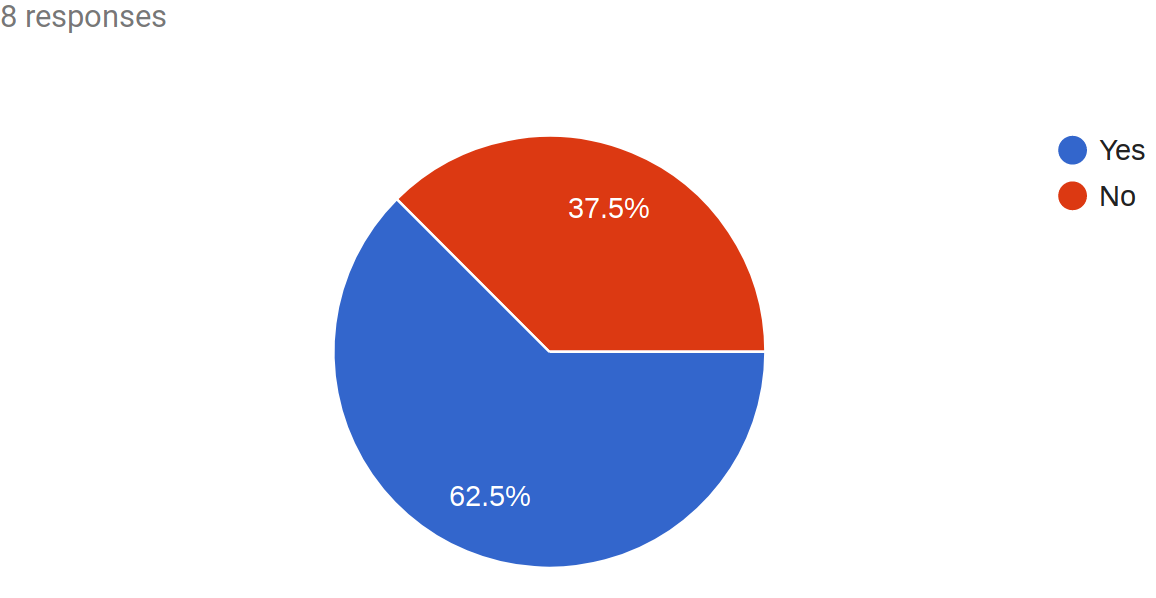
\includegraphics[width=0.8\linewidth]{figure/Evaluation/pie1.png}
	\caption{Pie chart showing visualizing whether or not the participants were able to do everything that the client wanted.}
	\label{fig:pie1}
\end{figure}

If the participant answered no, they had the ability to clarify further, such two comments were:\\

 \begin{quote}
 	
\textit{I had a hard time knowing where the client was on the glass plate compared to the items. Sometimes there were some consistency in where I placed the item and where it appeared, but I got the hang of it eventually}\\
  \end{quote}
  
  \begin{quote}
  \textit{Orientation is very difficult to understand}\\
  \end{quote}	
 	 
 	As it can be seen from the given answers, some of the participants had a hard time figuring out where the client was in the garden, which made it difficult for them to know where to place the objects in regards to the client.


\subsection{Findings}
In general the participants were positive about our prototype, the Likert scale questions showed an overall understanding of our prototype.
Especially in \autoref{fig:barChartEngaged} it can be seen that all 8 participants felt engaged with the program when they were in the VR environment. This could have something to do with the result of the question in \autoref{fig:barChartFrame}, a majority of the participants answered that the framerate was tolerable.\\


A fair amount of participants answered that they were able to do what the clients wanted as seen in \ref{fig:pie1}. A common statement from the participants were that it was difficult for them to localize the client in the garden. The architect couldn't see where the client was in the garden, because the client was able to move around freely inside the VR garden.\\


Over half of the participants answered that it was easy to follow the clients' instructions (see \autoref{fig:pie2}). Because we did not use a follow up question for this question we can't directly say why the last segment of participants had difficulties following the clients instructions.\\

Even though the above question was not elaborated further, the next given question, seen in \ref{fig:pie3} shows that half of the participants felt that the program responded to their actions, and half of them felt the opposite. This is very likely to have something to do with the prototype since some of the participants stated further that the prototype bugged out and didn't show the objects in VR. Another answer was that the objects didn't have any rotation, which might have made it more challenging for the participants to build the garden they had envisioned.



\section{Immersion test}
The immersion test was conducted to test how immersive our prototype was compared to two of the tools traditionally employed by garden architects, sketching and a 3D fly through. From the analysis in section \ref{sec:immersion} it was found that immersive virtual reality resulted in better spacial perception. As such, if our prototype feels more immersive it might be a better tool for presenting designs to clients.

\subsection{Test goals}
The goal of the test was to determine if the prototype in fact did answer the final problem statement (\autoref{sec:FPS}). The keywords from the FPS are:
\begin{itemize}
	\item[-] Fast
	\item[-] Efficient
	\item[-] Immersive
\end{itemize}
as such we were keen on measuring these usability goals in this test.
\subsection{Sampling}
Finding real garden architects among the students at AAU CPH, turned out to be a larger challenge, and therefore it was decided that convenience sampling were to replace that criteria. Convenience sampling among the students at AAU CPH gave us a "random" assortment of test participants. In total, twelve participants were found.
\subsection{Environment}
The test were carried out in our group room. The group members who were not part of the test would leave and work elsewhere during testing period. This was very much an artificial environment, again due to the difficulty getting a hold of target group memebers. The artificial environment allows do large quantities of tests, as we can bring participants into highly controlled situation and test very specific elements of the experience.
\subsection{Test specifics}
The participants were told they would be trying three different technologies, and were asked to try and understand they layout, in such a way that they could visualize it themselves. The participant were told to take as long as they needed with each of the parts. The parts consisted of:
\begin{itemize}
	\item[-] 2D sketching
	\item[-] 3D viewing
	\item[-] Virtual reality
\end{itemize}
After each part a four question questionnaire of Likert scales was filled out, that can be seen in \todo{but questionnaire in appendecies} . This meant that each person would answer the same questionnaire three times. From this we would be able to see how the testers rated the different parts in terms of immersiveness, speediness of spacial understanding, perceived usefulness to garden architects, and understanding of the gardens design. To differentiate between the subjects they were each given a participant number. As each participant spend longer time observing the garden, we predicted their understanding would improves. To eliminate this bias we used every possible sequence combination of 2D sketching, 3D viewing and Virtual Reality on two differently designed gardens, as seen in \autoref{table:immersionCombinations}.

\begin{table}[H]
	\centering
	\caption{All the sequence combinations of 2D sketching, 3D viewing and virtual reality, and which participant that did what combination.}
	\label{table:immersionCombinations}
	\begin{tabular}{l | c|c|c|c|c|c}
		&
		\begin{tabular}[c]{@{}c@{}}VR\\ 2D\\ 3D\end{tabular} & \begin{tabular}[c]{@{}c@{}}VR\\ 3D\\ 2D\end{tabular} & \begin{tabular}[c]{@{}c@{}}2D\\ 3D\\ VR\end{tabular} & \begin{tabular}[c]{@{}c@{}}2D\\ VR\\ 3D\end{tabular} & \begin{tabular}[c]{@{}c@{}}3D\\ VR\\ 2D\end{tabular} & \begin{tabular}[c]{@{}c@{}}3D\\ 2D\\ VR\end{tabular} \\ \hline 
		Garden 1 & 2                                                                            & 5                                                                            & 4                                                                            & 3                                                                            & 1                                                                            & 6                                                                            \\ 
		Garden 2 & 7                                                                            & 8                                                                            & 9                                                                            & 10                                                                           & 11                                                                           & 12                                                                           \\
	\end{tabular}
	
\end{table}
The 2D sketches the participants were asked to study can be seen in \autoref{fig:sketchGarden1} and \autoref{fig:sketchGarden2}. These were both created from the 3D virtual scenes made in unity. The two gardens purposely have two very different layouts, and two very different complexity levels(The number of objects in the scene). This was done in an attempt to eliminate bias and the odds of the results being up to chance, as one layout might favor one part.
\begin{figure}[H]
	\centering
	\begin{minipage}[b]{0.49\textwidth}
	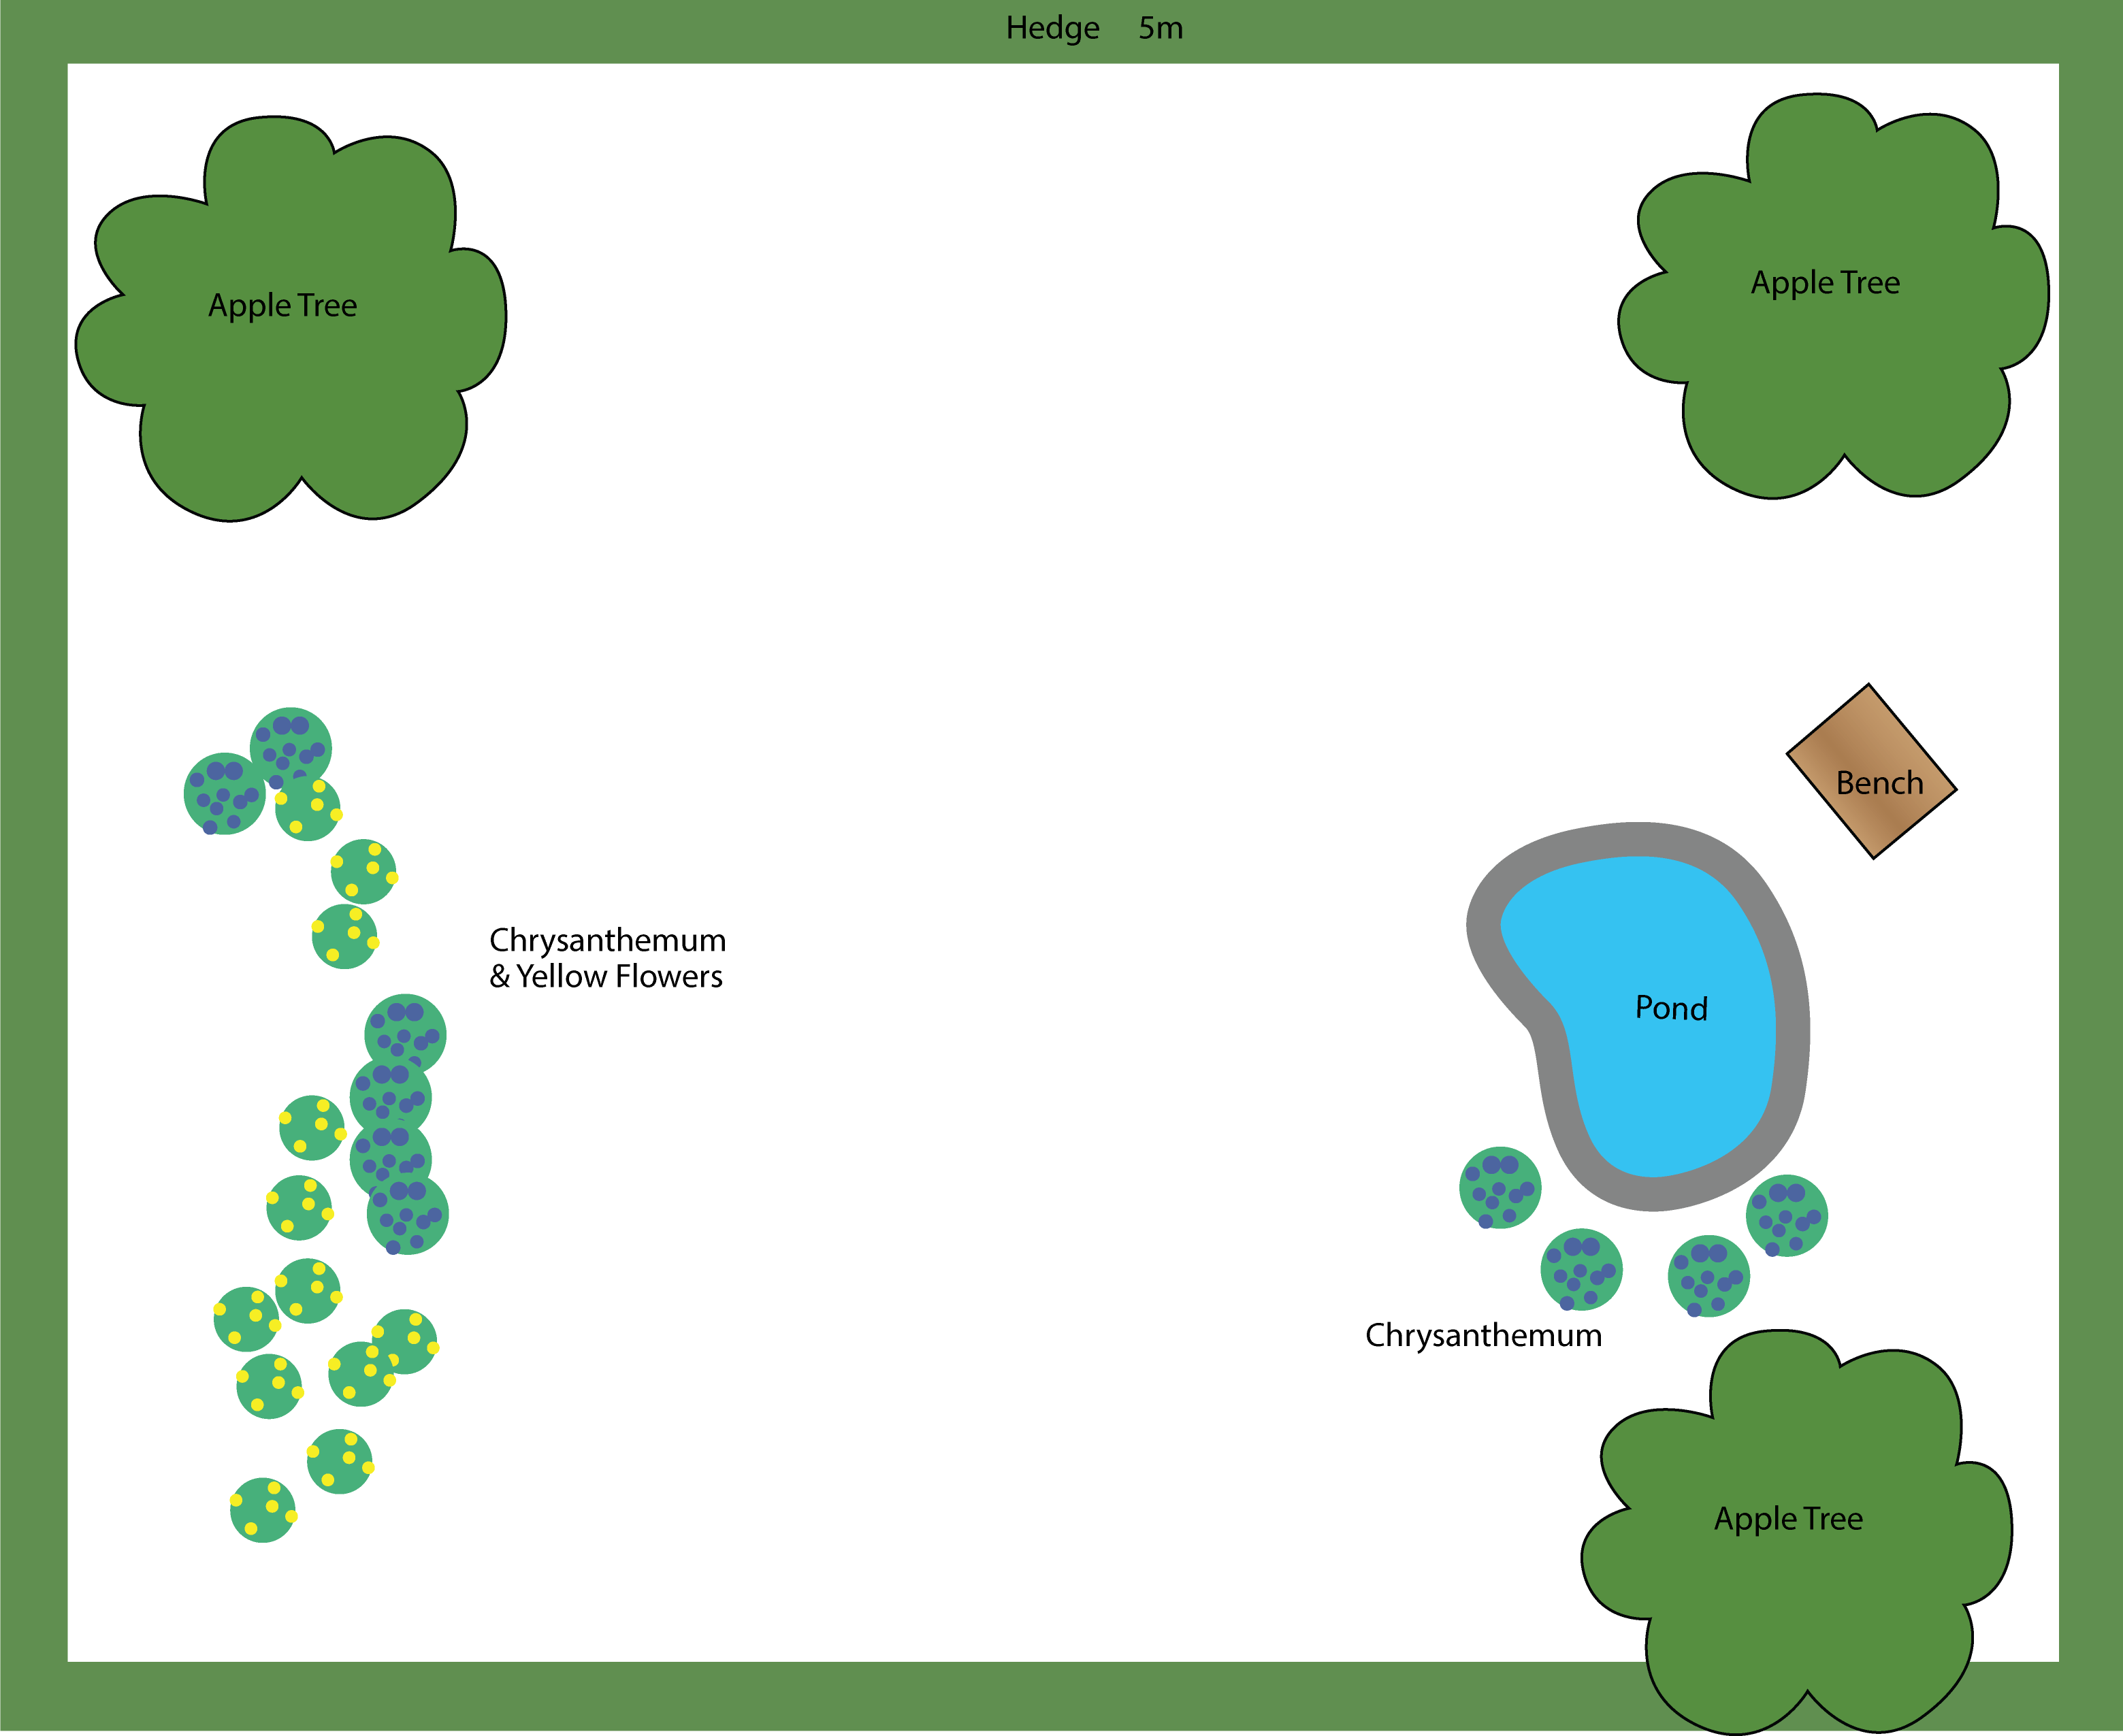
\includegraphics[width=1.0\linewidth]{figure/Evaluation/Garden1.png}
	\caption{Sketch garden 1}
	\label{fig:sketchGarden1}
	\end{minipage}
	\hfill
	\begin{minipage}[b]{0.49\textwidth}
	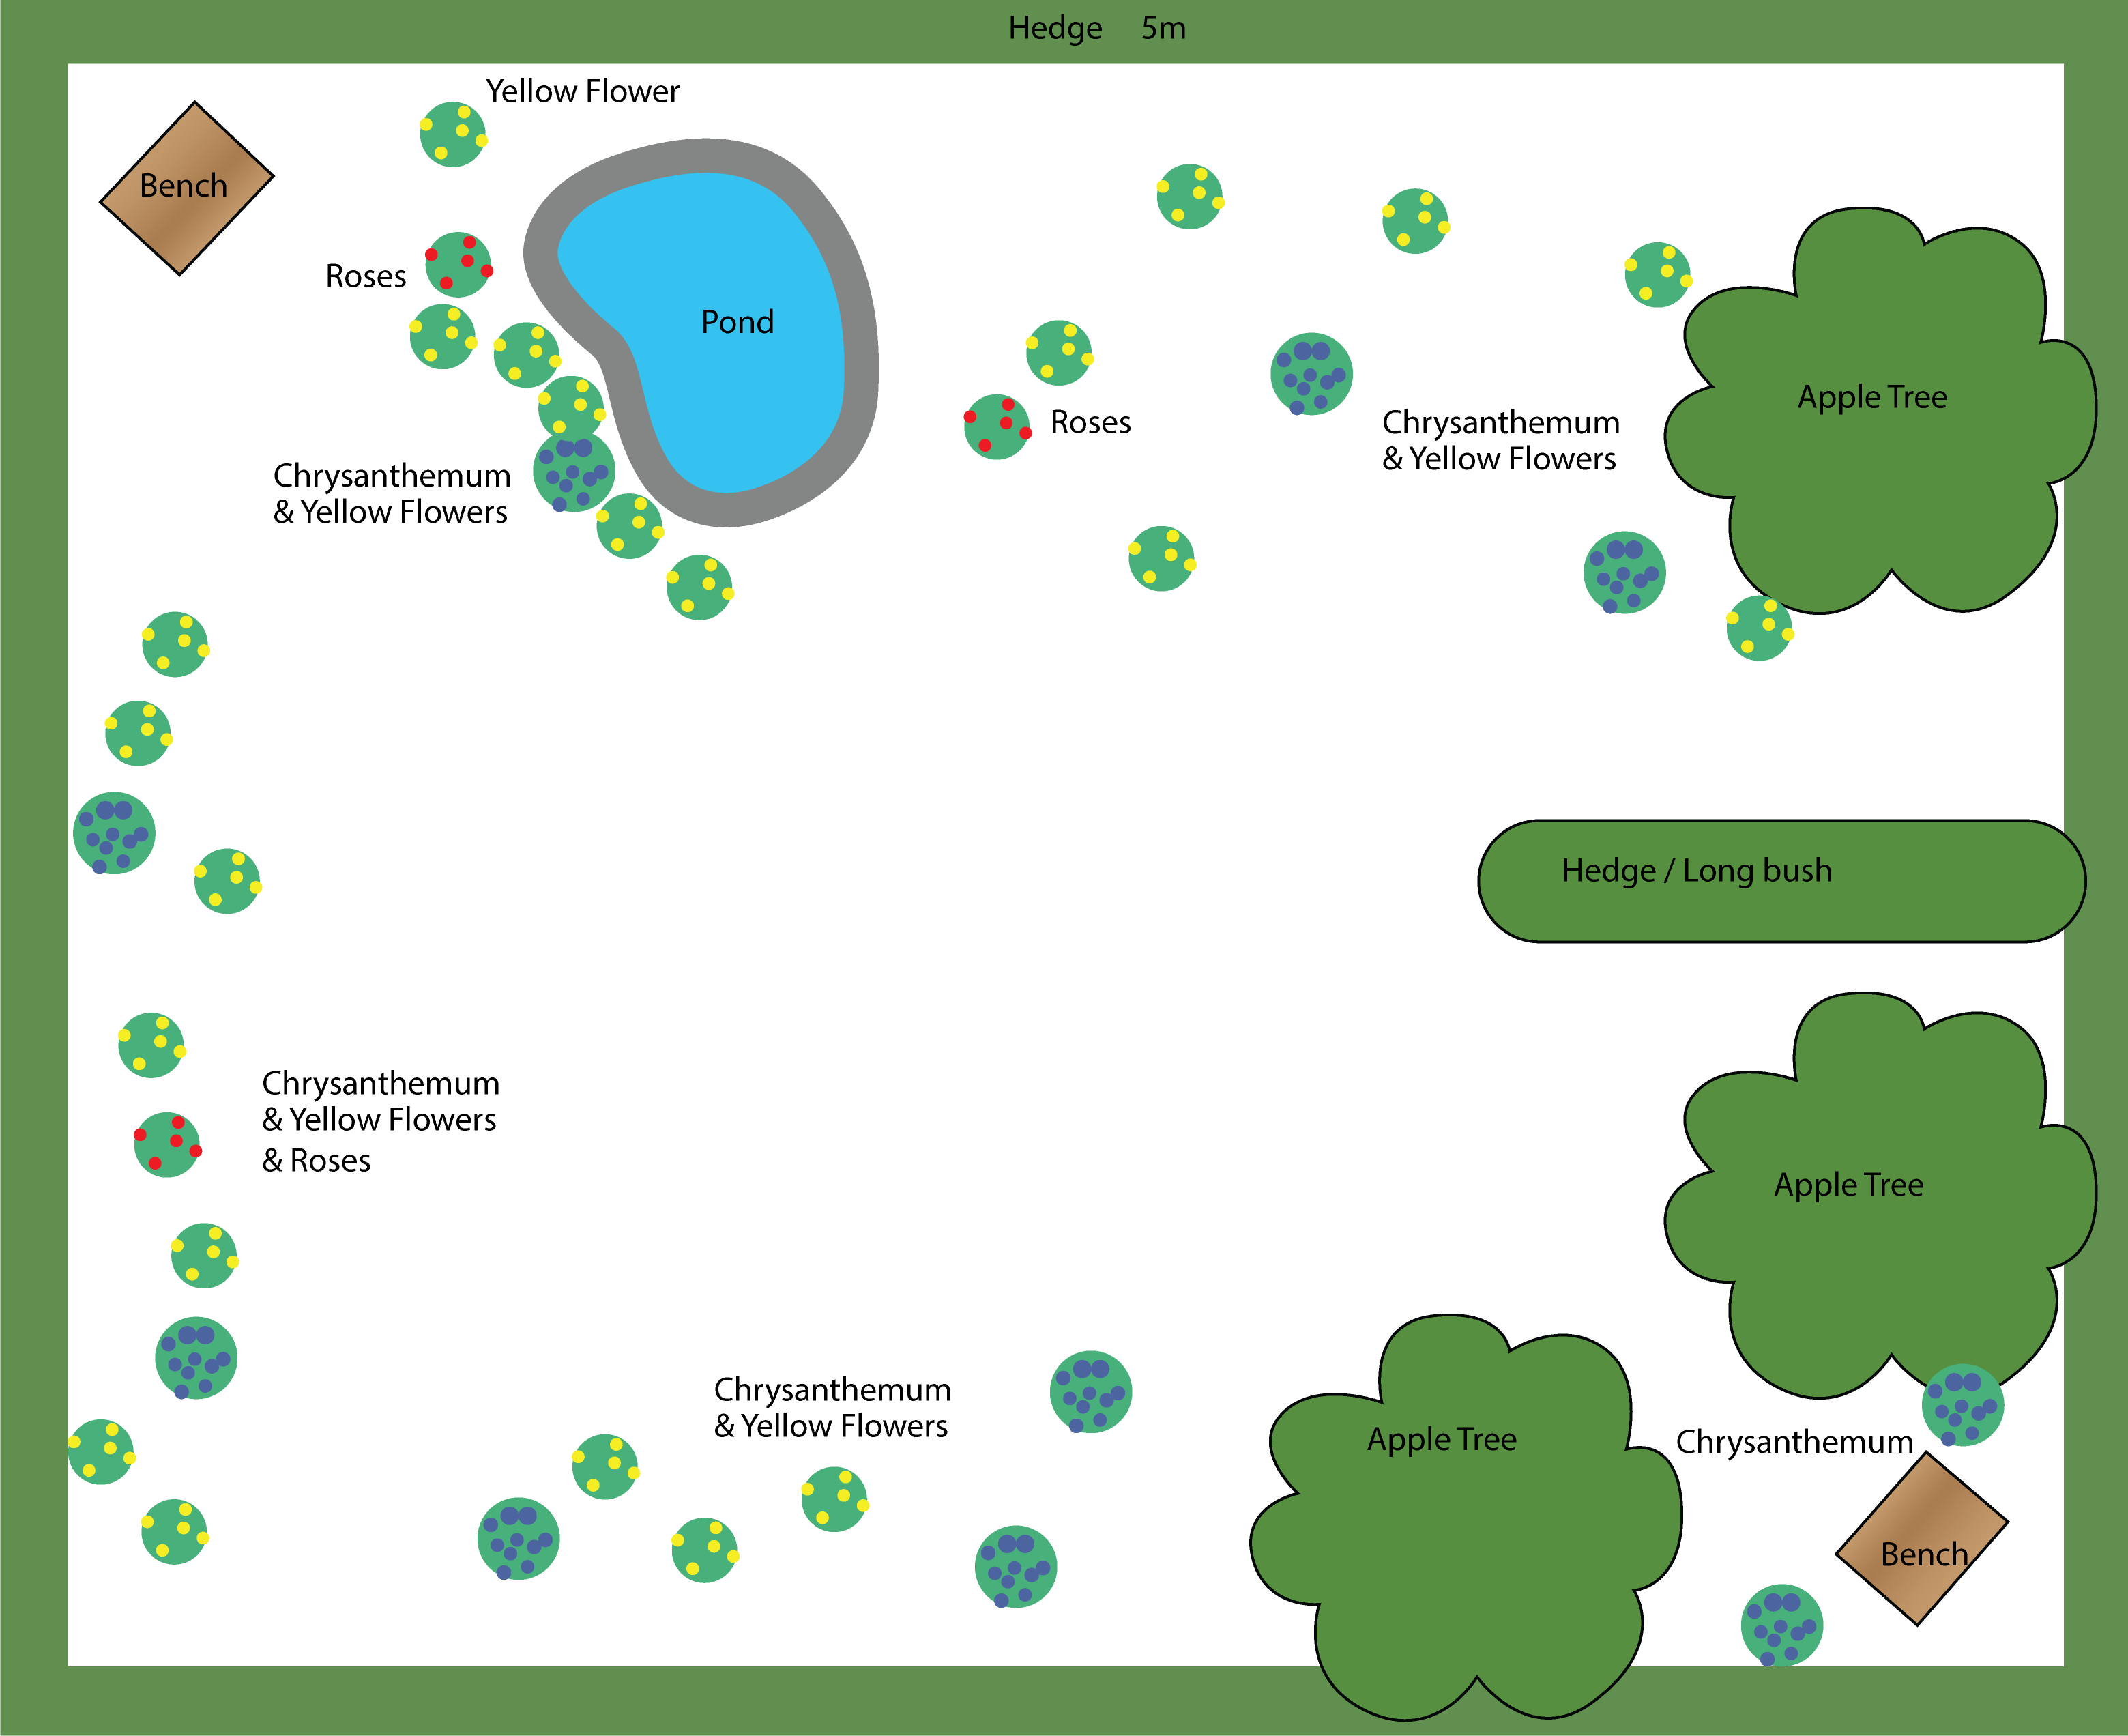
\includegraphics[width=1.0\linewidth]{figure/Evaluation/Garden2.png}
	\caption{Sketch garden 2}
	\label{fig:sketchGarden2}
	\end{minipage}
\end{figure}
The 3D scenes had a camera that automatically moved and looked around the garden. This was done to replicate what we observed some garden architects were advertising on their web pages\footnote{Visualization done by garden architect : \url{https://youtu.be/1ki9H5fs7EI}}. In VR, the participants could use the controller to teleport around and observe the garden, as described in Section \ref{sec:designUI}. 

\subsection{Findings}
After the tests had finished, we compiled the answers into two tables, one for garden 1 (\autoref{table:averageResponseGarden1}) and one for garden 2 (\autoref{table:averageResponseGarden2}). These tables contained the averages of the responses.
\begin{table}[H]
	\centering
	\caption{Average of responses with test on garden 1, higher numbers are better}
	\label{table:averageResponseGarden1}
	\begin{tabular}{p{3cm}|p{3cm}|p{2cm}|p{3cm}|p{3cm}}
		Test type       & How long do you think it took you to gain insight into how it would be, to be in the garden? & How immersed did you feel? & How useful do you think this tool could be for a garden architect? & How much do you feel like you understood the garden's design? \\ \hline
		&&&&\\
		Sketching       & 6.75    & 2.00    & 3.92      & 7.58            \\
		3D Viewing      & 6.08  & 4.67  & 4.00    & 8.67               \\
		Virtual Reality & 8.17     & 7.67     & 4.58      & 9.17    
	\end{tabular}
\end{table}
From \autoref{table:averageResponseGarden1} it can be be seen that for all four questions, Virtual reality was rated higher than when 3D viewing and 2D sketching. For the first question, about the length of time it took the participant to gain insight into how it would be, to be in the garden, in both garden 1 and 2, the participants rated virtual reality as the quickest (Higher number is faster). In both gardens however, the 3D viewing experience was rated the slowest (6.08 and 5.50).
\begin{table}[H]
	\centering
	\caption{Average of the responses with test on garden 2, higher numbers are better}
	\label{table:averageResponseGarden2}
	\begin{tabular}{p{3cm}|p{3cm}|p{2cm}|p{3cm}|p{3cm}}
		Test type       & How long do you think it took you to gain insight into how it would be, to be in the garden? & How immersed did you feel? & How useful do you think this tool could be for a garden architect? & How much do you feel like you understood the garden's design? \\ \hline
		&&&&\\
		Sketching       & 7.00                                                                                         & 2.33                       & 4.00                                                               & 8.00                                                          \\
		3D Viewing      & 5.50                                                                                         & 4.67                       & 3.83                                                               & 7.83                                                          \\
		
		Virtual Reality & 8.00                                                                                         & 6.17                       & 4.50                                                               & 8.67                                                         
	\end{tabular}
\end{table}

In general, when asked about how immersed the participants felt during the test, they picked much higher numbers in garden 1 than garden 2, we believe this to be down to the difference in complexity between the two gardens, as garden 2 have substantially more objects in the scene, and is therefore more complex to understand.
The question about immersiveness was on a scale from 1 to 10, and generally 2D sketching wasn't making the participants feel immersed, while Virtual reality on the other hand, in garden 1, was almost ranked 4 times higher.\\\\

Usefulness was rated on a scale on from 1 to 5, and overall usefulness is rated high, with the lowest average being 3D viewing in garden 2, rated at 3.83. This question was designed to make the participant take the standpoint of a garden architect, and hence try to visualize the usefulness of each tool in the hypothetical work flow.\\
To better get an idea of whether or not the participant could understand the garden they were seeing, they were asked to rate their own understanding of the garden's design on a scale from 1 to 10. Just like the usefulness response, all of the answers were quite high, with the lowest being 7.58, for sketching in garden 1.\\

All but 1 participant answered the final question prompting a comparison between the three different mediums. 
The contents of the comments have been separated into statements about the individual mediums:
\subsection*{3D viewing}
	8 out of 12 participants left a comment on what could be changed for 3D viewing. Of those, 7 comments concerned the ability to navigate or interact with the environment themselves. One comment said it would be beneficial to see the dimensions of the objects in the garden. A list of the condensed comments in in descending order can be seen in \autoref{table:condensed3D}.
		\begin{table}[H]
		\centering
		\caption{Comments about the 3D viewing, condensed into categorized statements}
		\label{table:condensed3D}
		\begin{tabular}{p{5cm}|c}
			Comment & Count \\ \hline
			Bad to not have control & 3 \\
			Some immersion & 3 \\
			Fast overview &2 \\
			Lacking some immersion &2 \\
			Felt polished& 1 \\
			Lack of dimensions& 1 \\
			Good for angles& 1 \\
			Lack of depth perception& 1 \\
			Movement confusing& 1 \\
			Strange& 1 \\
			Good idea of layout& 1 \\
		\end{tabular}
	\end{table}
\subsection*{2D Sketching}
	Of the sketching comments, 9 of 12 testers left a comment. Five comments said they wouldn't change anything or didn't know what they'd change. Two comments said they needed more depth to the image. One tester wanted a more detailed sketch, and one asked for a "more immersive experience" The tester who left the last comment started with the 2D sketch as the first medium for visualization and may have found the immersion question silly without any other medium to compare it to. A list of the condensed comments in descending order can be seen in \autoref{table:condensed2D}.
	\begin{table}[H]
		\centering
		\caption{Comments about the 2D sketching, condensed into categorized statements}
		\label{table:condensed2D}
		\begin{tabular}{p{5cm}|c}
			Comment & Count \\ \hline
			Quick & 3 \\
			Descriptive & 2\\
			Not immersive & 2 \\
			Good for accurate positions & 2 \\
			Good overview  & 2 \\
			Easy to understand & 2 \\
			Difficult to visualize & 1 \\
			Inaccurate& 1 \\
			Good for sizes & 1 \\
		\end{tabular}
	\end{table}
\subsection*{Virtual Reality}
	As for the Virtual Reality test, 9 out of 12 testers left a comment. 1 of the 9 didn't know what could be improved. 1 person wanted elements like floor plans. Two wanted improved graphics. One person wanted a note taking functionality, the ability to highlight objects, and multi-user functionality. Two users wanted more interactivity, and two users wanted a larger area to walk around, as to remove the need for teleportation. A list of the condensed comments in descending order can be seen in \autoref{table:condensedVR}.
	\begin{table}[H]
		\centering
		\caption{Comments about the virtual reality, condensed into categorized statements}
		\label{table:condensedVR}
		\begin{tabular}{p{5cm}|c}
			Comment & Count \\ \hline
			Good for immersion & 7 \\
			Good feel of garden & 4 \\
			Good for size  & 2 \\
			Useful & 2 \\
			Lacking interactivity & 2 \\
			Good for angles & 1 \\
			Good for distances& 1 \\
			Lack of dimensions& 1 \\
			Good for focus on detail& 1 \\
			Limited FOV& 1 \\
			Natural& 1 \\
			Interesting& 1 \\
			Quick insight& 1 \\
			Low FPS& 1 \\
			Lack of overview& 1 \\
			Good for layout& 1 \\
			
		\end{tabular}
		
	\end{table}

